\section{Solution Design}

This section will describe the solution in terms of the distributed and
concurrent parts of the system and the communication protocols that we have
designed:

\begin{itemize}
\item \textbf{Concurrency -- Application Layer}:
  description of application-layer communication protocols. In this section we
  will expose the reason why certain protocols have been chosen and which
  properties they are able to guaranteed for the communication of the system
\item \textbf{Distribution -- Middleware Layer}:
  in a very similar way as the previous point, we will clarify which protocols
  we established for the middleware to behave as wished;
\item \textbf{Distribution -- Broker}:
  we will say just a couple of words about our message broker works;
\item \textbf{Artificial Intelligence (AI)}:
  description of how we solved the problem of computing each agent's path
  in a distributed, multi-agent, dynamic environment.
\end{itemize}

% Communication Protocols subsection
\subsection{Application}
The Application is composed of two different sub-components (Figure
\ref{fig:sd-app-init}):

\begin{itemize}
  \item \textbf{Application Logic Layer}: handles the application logic
    (slightly abusing the notation, we will often refer to it simply as
    \textit{Application Layer});
  \item \textbf{Interface Layer (IL)}: provides the remote services to Application
    Layer by acting as an interface towards the underlying middleware layer.
\end{itemize}

In the next sections we will use the following terms to describe the state of a
software layer or a package:
\begin{itemize}
	\item \verb|inactive| - not even created;
	\item \verb|ready| - initialized with all the needed resources. Not yet
	allowed to execute;
	\item \verb|active| - executing;
	\item \verb|stopped| - not executing. It is waiting to terminate.
\end{itemize}

\subsubsection{Application Layer}\label{sec:sol-des-app-layer}

\input{sections/solutionDesign/architecture/app-layer/entityType.tex}



Figure \ref{fig:sd-app-backend-architecture} provides an architectural overview
of the main classes which compose the application layer.
As shown in the figure, the core packages have been named according to
Table \ref{tab:entity_type}.

\begin{figure}[H]
  \centering
  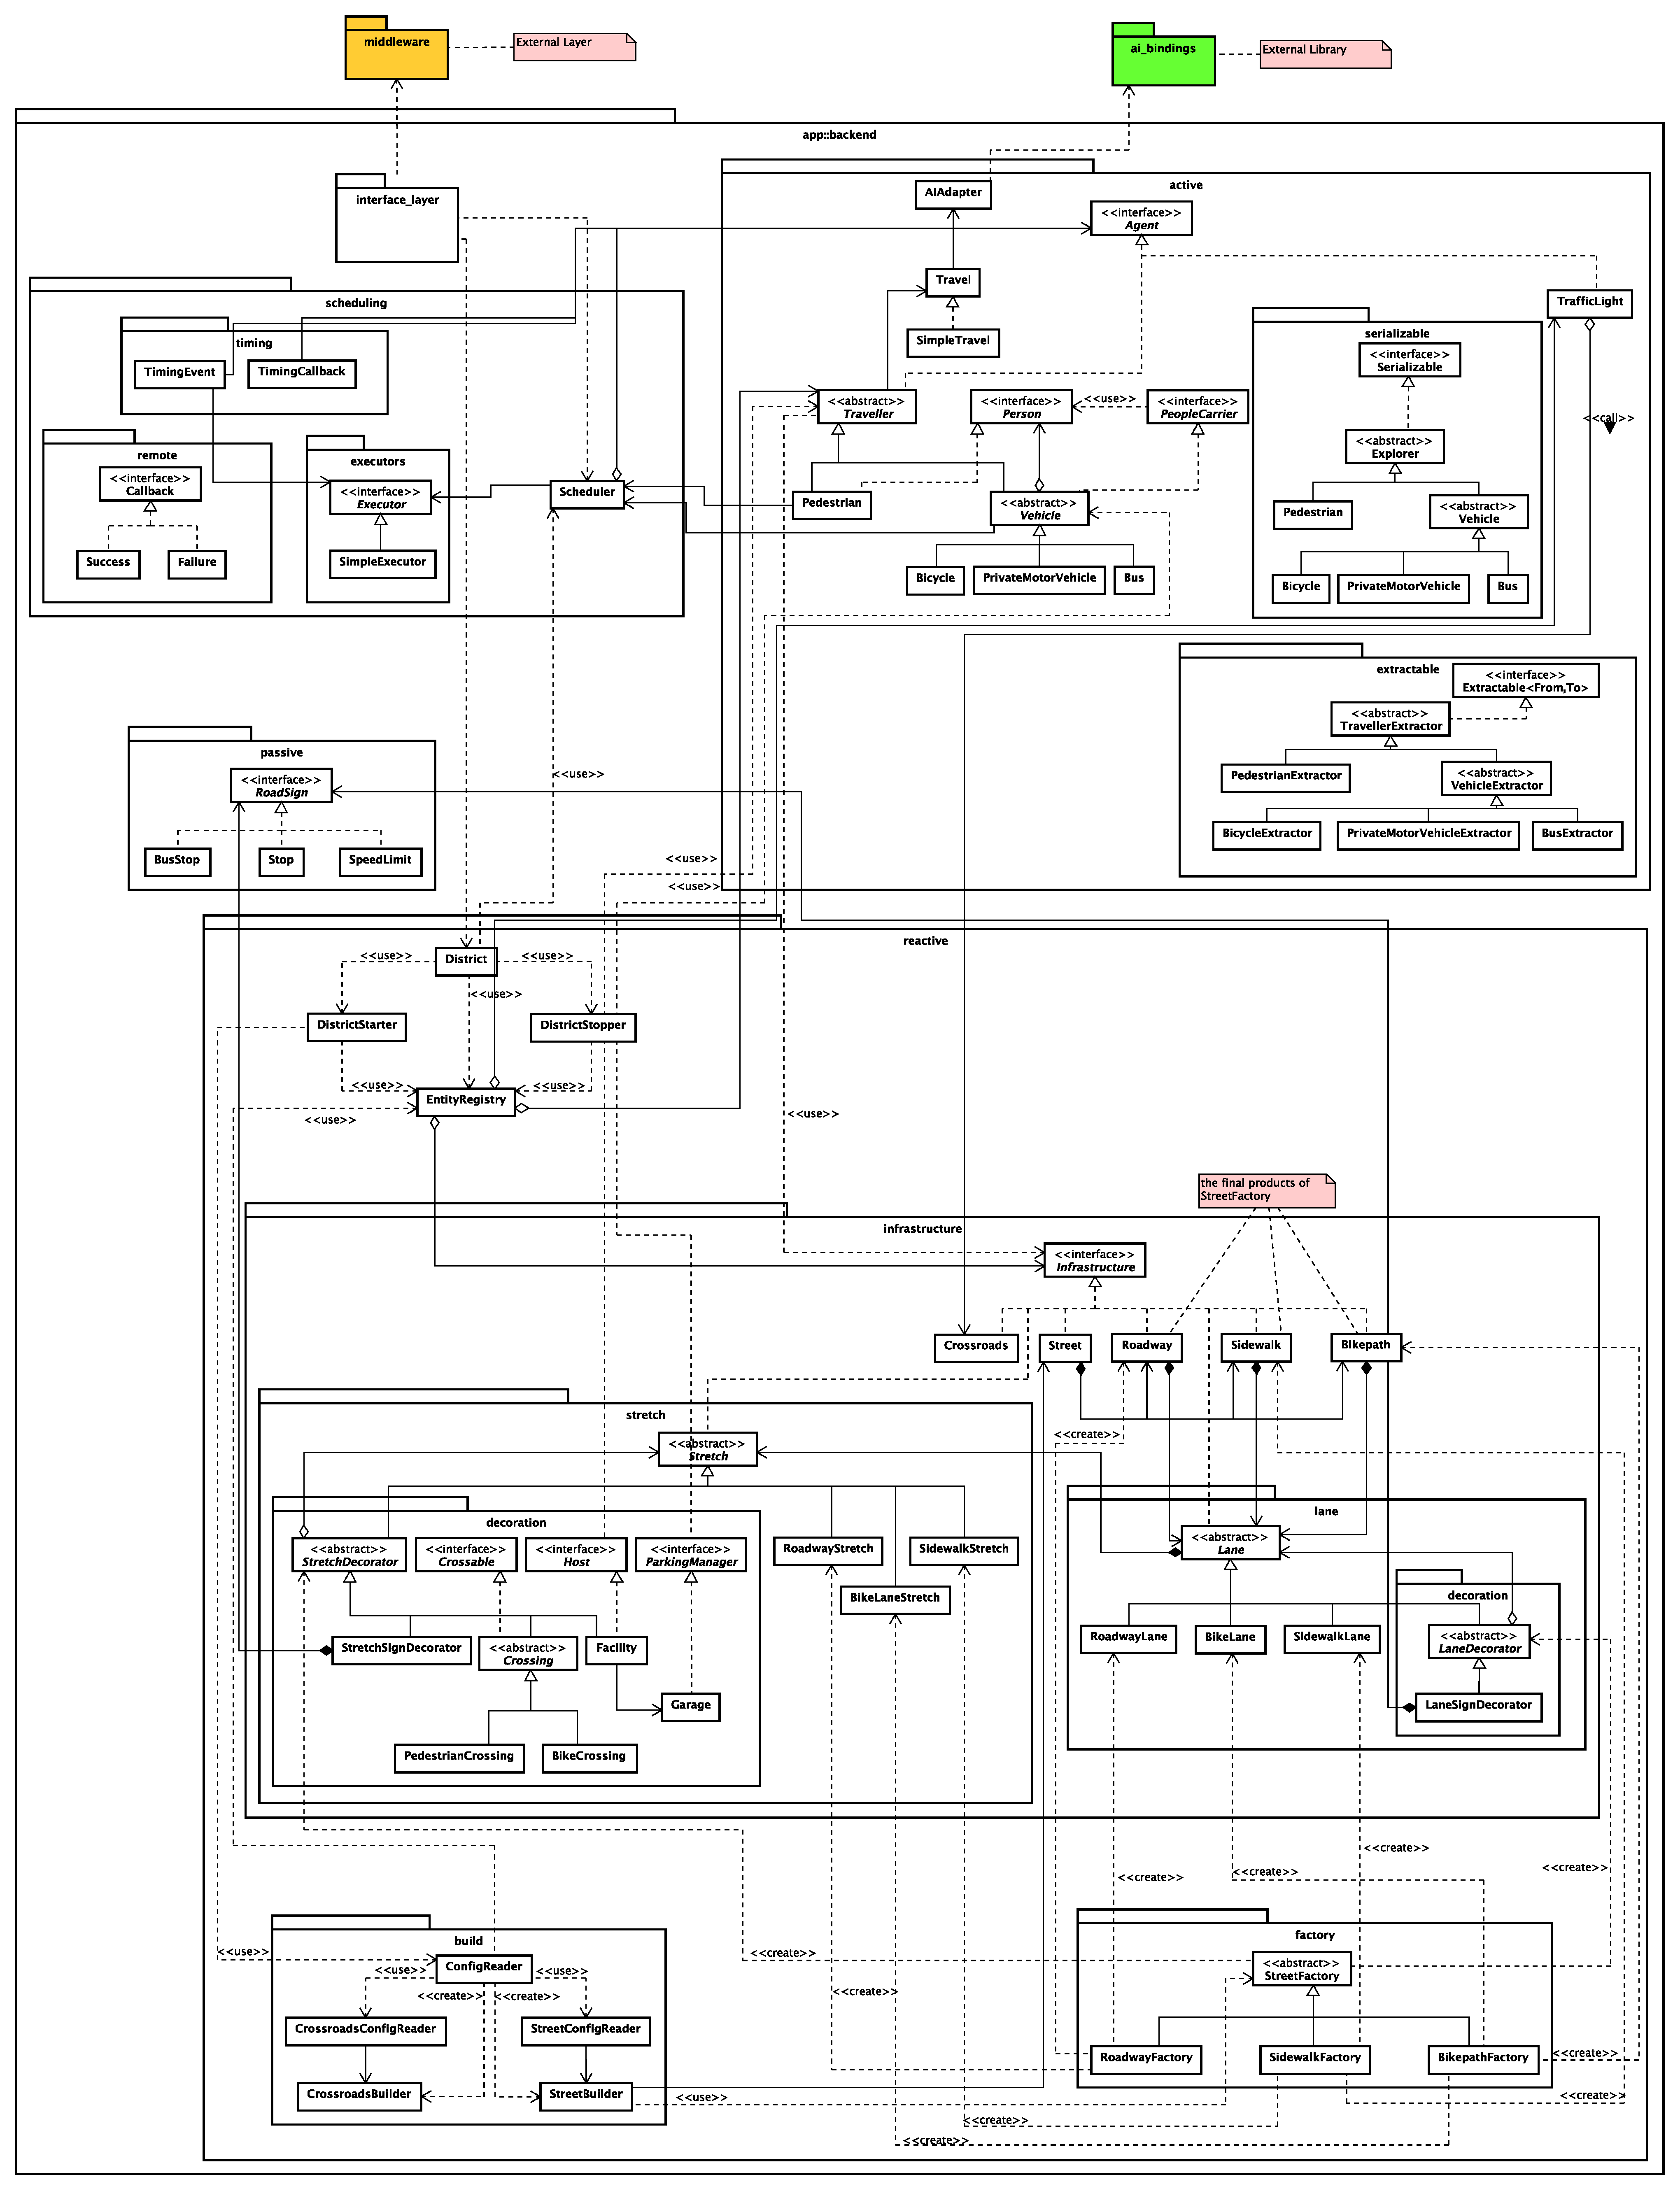
\includegraphics[width=.95\columnwidth]{images/solution/app/backend/app_backend_architecture.eps}
  \caption{Application Layer: top level design}
  \label{fig:sd-app-backend-architecture}
\end{figure}

\input{sections/solutionDesign/architecture/app-layer/active.tex}
\input{sections/solutionDesign/architecture/app-layer/reactive.tex}
\input{sections/solutionDesign/architecture/app-layer/passive.tex}
\input{sections/solutionDesign/architecture/app-layer/scheduling.tex}
\subsubsection{Artificial Intelligence (AI)}

To solve the path
problem outlined in Section \ref{sec:pa-distribution}
we have implemented a path-finder for the agents of our system.
Our AI is written in C++ but we have written the Ada bindings for it.
Thus, being able to statically link the AI to our project.

The path-finder is executed by the ACTS scheduler. In particular, a
worker runs the \verb|agent.act| procedure which contains invocations
to AI.

% The AI needs to know on which graph/infrastructure the agent
% is traveling on. Indeed, different travelers moves on different
% infrastructures. For example, a car needs to travel only on roads which are
% mostly
% separated from other city infrastructures. Thus, the AI maintains three
% search graphs, one for each infrastructure (roads, bicycle paths, sidewalks).
% In case of intersection or crossing stretches, the ids (of the stretches)
% are replicated over different graphs.


\subsubsubsection{Environment}

The first step when planning an AI consists in analyzing the task environment
to clearly understand the problem:

\begin{itemize}

\item{deterministic} -
the next state is completely defined by the previous state plus the move
performed by the agent;

\item{discrete} -
there are many state of the system, but their number is finite.
The agent acts in a discrete space and the information which he manipulates
are also discrete (e.g., costs of moves);

\item{sequential} -
the choice of the next move depends on the previous one. The agent creates
a totally ordered sequence of moves;

\item{dynamic} -
the environment change around the agent while he is computing its moves;

\item{multi-agent} -
there are several agent who act concurrently in the same virtual
environment;

\item{partially observable} -
since the system is distributed, the agent does not have access to the complete
information about the whole environment. At any time, an agent is
traveling on a
specific district which has only updated information on its state and does not
know the costs of the other districts. Also, an agent eventually needs to
compute a path which comprise several districts.
\end{itemize}

\subsubsubsection{Search algorithms}

Due to time constraints related to the path computation, we preferred to
choose a not-real-time solution. However, we recognize that a real-time solution
helped by a traffic forecast model would be more precise and interesting.
Our solution uses classical path-finding algorithms. These algorithms
belong to uninformed and informed search classes.

Our AI offers three path finding algorithms:
\begin{itemize}
  \item Greedy Search;
  \item Uniform Cost Search;
  \item A* Search.
\end{itemize}

The first one is incomplete and not optimal because of the local search which
looks only one step ahead (visiting
only the neighbors). The last two algorithm are both complete and optimal
under certain assumptions. They have been defined
to guarantee our agents to always find the best possible path with
the minimum number of visited nodes in the search graph.

\subsubsubsection{Properties}

To guarantee completeness we need to assume that each graph is a strongly
connected component. Basically, it means that there are no isolated
components. Thus, the agent knows there will always be at least a path between
the source and the destination of its plan. % its or her
\\

Furthermore, our AI considers not grid based maps: which means some common
heuristics are not applicable a priori (e.g. Manhattan distance, euclidean
distance). Also, since grid-based maps are a subset of all possible maps, we
can say that our AI is independent on the map topology.
\\

To solve the path finding problem we reason about the specific domain and its
abstractions in terms of infrastructure building blocks and travelers. We
found an admissible and consistent heuristic for A* and, more in general, other
informed algorithms. To concretely guarantee the assumptions hold for all the
graph configurations we apply the Tarjan algorithm to each of them.
\\

Tarjan automatically validates our graphs at build time by ensuring that there
is only one strong connected component for each graph. Otherwise, it reports
an error and the isolated component.
Finally, the AI is agent-independent, which means we can use it to calculate
the path of different kinds of agents: bicycles which move on bicycle lanes,
pedestrians who move on sidewalks and motor vehicles which move on roads.
Thus, each infrastructure is represented by a different infrastructure graph.
Overall, the AI manipulates three infrastructure graphs plus N costs graphs
which represent the traffic costs of a specific district.

\subsubsubsection{Heuristic}

We have approximate the dynamic component of the environment by considering
the state of the system during the simulation as a sequence of snapshots.
Thus, each snapshot can give to the path-finder the information it needs
about the city traffic.
This information is detected by a daemon process which belongs to the AI.
It uploads new generated graphs of the dynamic costs (the costs of the traffic)
in the AI graph registry. The daemon action is triggered each time a new
snapshot is generated.
\\

The traffic costs are computed as the number of agents which are on a specific
stretch when the snapshot is performed. Also, the intersections have an additional
cost given by the traffic lights which can slow down the travel of the agent.
\\

Unfortunately, the system
snapshots were not provided as planned at the beginning of the project, so
the AI computes paths always on the same infrastructure graph without
considering the traffic costs. However, its effectiveness (with traffic costs)
has been proved by running it on a city written in NodeJS for another
proof of concept simulator.

\subsubsection{Interface Layer}

Figure \ref{fig:impl-il-arch} provides an high level view of
the Interface Layer (IL) components.

\begin{figure}[H]
  \centering
  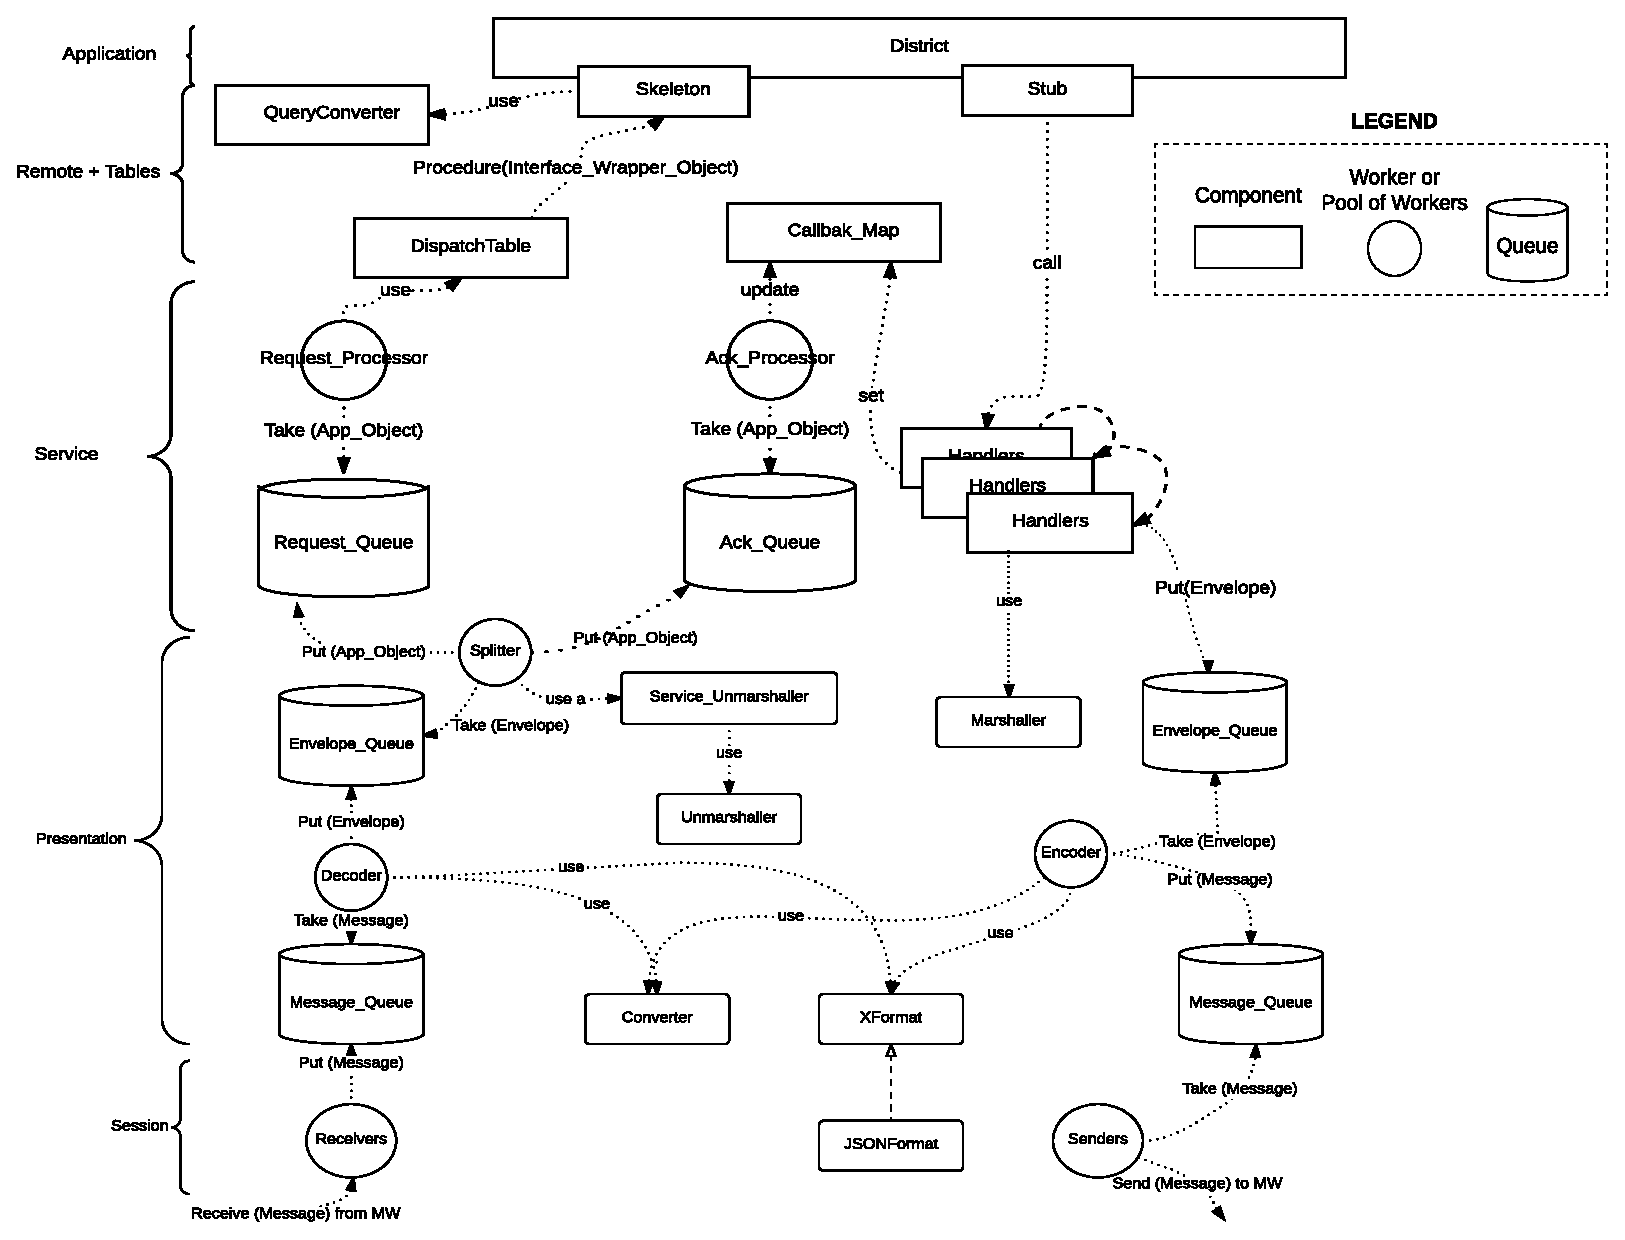
\includegraphics[width=\columnwidth]{images/solution/il.eps}
  \caption{Interface Layer architecture}
  \label{fig:impl-il-arch}
\end{figure}

IL enables the Application Layer to communicate with other applications
transparently without knowing if they are local or remote. We encapsulate the
application data as message payload while
different sublayers of IL manipulate different fields of the
message header.
This layered approach has been inspired by the TCP/IP and ISO/OSI models, in
which the layers communicate in two directions:
\begin{itemize}
	\item \textbf{horizontally:} manipulating the same fields of the header;
	\item \textbf{vertically:}  - passing the packet to the next
layer, which is charged with different responsibilities.
\end{itemize}
Also, IL is completely asynchronous because each of its sublayers has its own
thread pool. Furthermore, each thread pool is controlled by a master thread which
runs in an event loop consuming messages from its own incoming
queue. For example, the receiver can handle potentially multiple concurrent
requests by delegating each one of them to its worker threads.
After a worker has
completed the assigned task it is pushed back on the receiver's local stack,
ready to be reused.


In the following we list the sublayers which compose IL in
bottom up order:

\begin{itemize}
  \item \textbf{Session Layer:}
  handles remote connections through TCP sockets;
  \item \textbf{Presentation Layer:}
  handles messages formatting and conversions;
  \item \textbf{Service Layer:}
  converts remote requests into procedure calls
  by leveraging a skeleton object.
  Also, it offers the specular service through a stub object plus a pipeline
  of handlers. For each request, the former compose a specific pipeline
  of handlers transparently to the Application Layer.
  The handlers are used to incrementally construct the message by adding
  header fields, wrapping the data into a payload field and finally putting
  the message in the first queue which goes downwards (towards the middleware).
  \item \textbf{Remote Layer + Tables:}
  It contains the tables used
  to dispatch the remote calls and the callback map of pending requests.
  A pending request is a synchronous requests which may trigger one of
  the following behaviors:
  \begin{itemize}
  	\item retransmission on timeout;
  	\item a local retry on failure - retry on the local district with
  	the next action which could be a repetition of the last executed action;
  	\item a local clean up on success - remove the retained data from the local
  	district. The message has been successfully sent.
  \end{itemize}
  With pending request we are not reinventing a weakened version
  of TCP retransmission timers as it might seem.
  Indeed, we have concretely faced network connection errors during
  the communication
  with the middleware layer. This was caused by occasional failures or network
  problems subsequently fixed by the system itself
  (i.e., the docker swarm node).
  However,
  we preferred to give the responsibility of these synchronous messages to IL
  for two reasons:
  \begin{itemize}
  	\item it is the layer which has the highest probability of not losing them.
  	Indeed, the communication with the Application Layer happens through
  	local procedure
  	calls. Also, the TCP communication with the middleware layer could lead to
  	lose messages;
  	\item the data wrapped in the messages are important for the
  	application which can not afford to lose them. Indeed, a lost message
    could mean a missing pedestrian in the system. Thus, a failure
  	or a timeout has to trigger a reaction as soon as possible because
  	the latency introduced in the communication can lead to a significant
  	time drift for the end user (e.g., a set of travelers blocked with
  	apparently no reason). This could undermine the principle of viewing the
  	whole distributed system as one single unit.
  \end{itemize}
\end{itemize}
\subsubsection{Bootstrap}

The bootstrap process consists of two ordered and separated processes:

\begin{enumerate}
  \item \textbf{Initialization:} instantiates and configures the necessary
    resources for the application;
  \item \textbf{Activation:} starts the application.
\end{enumerate}

Clearly, the activation phase depends on initialization.
While the initialization process is automatically triggered at node creation,
this is not the case for activation, which is instead triggered by the
middleware.
Moreover, at the Application Layer level, we have to consider the dependencies
among the entity types (which are depicted in Figure
\ref{fig:sd-entity-types-deps}).

The overall bootstrap process, which mimics UNIX init \cite{online-tlsag},
is divided in two ordered parts:
\begin{enumerate}
  \item \textbf{Init:} initialize all the sublayers of each macro layer,
  following a bottom up approach (from \verb|interface_layer.session| to
  \verb|application.scheduling|).
  The initialization order is given by the fact that the upper
  layers need the services provided by the underlying layers to work
  correctly (Figure \ref{fig:sd-app-init});
  \item \textbf{Start:} IL forwards the start message sent from the
  middleware to the Application Layer.
  Therefore, this event is exclusively triggered by the middleware.
\end{enumerate}

\begin{figure}[H]
  \centering
  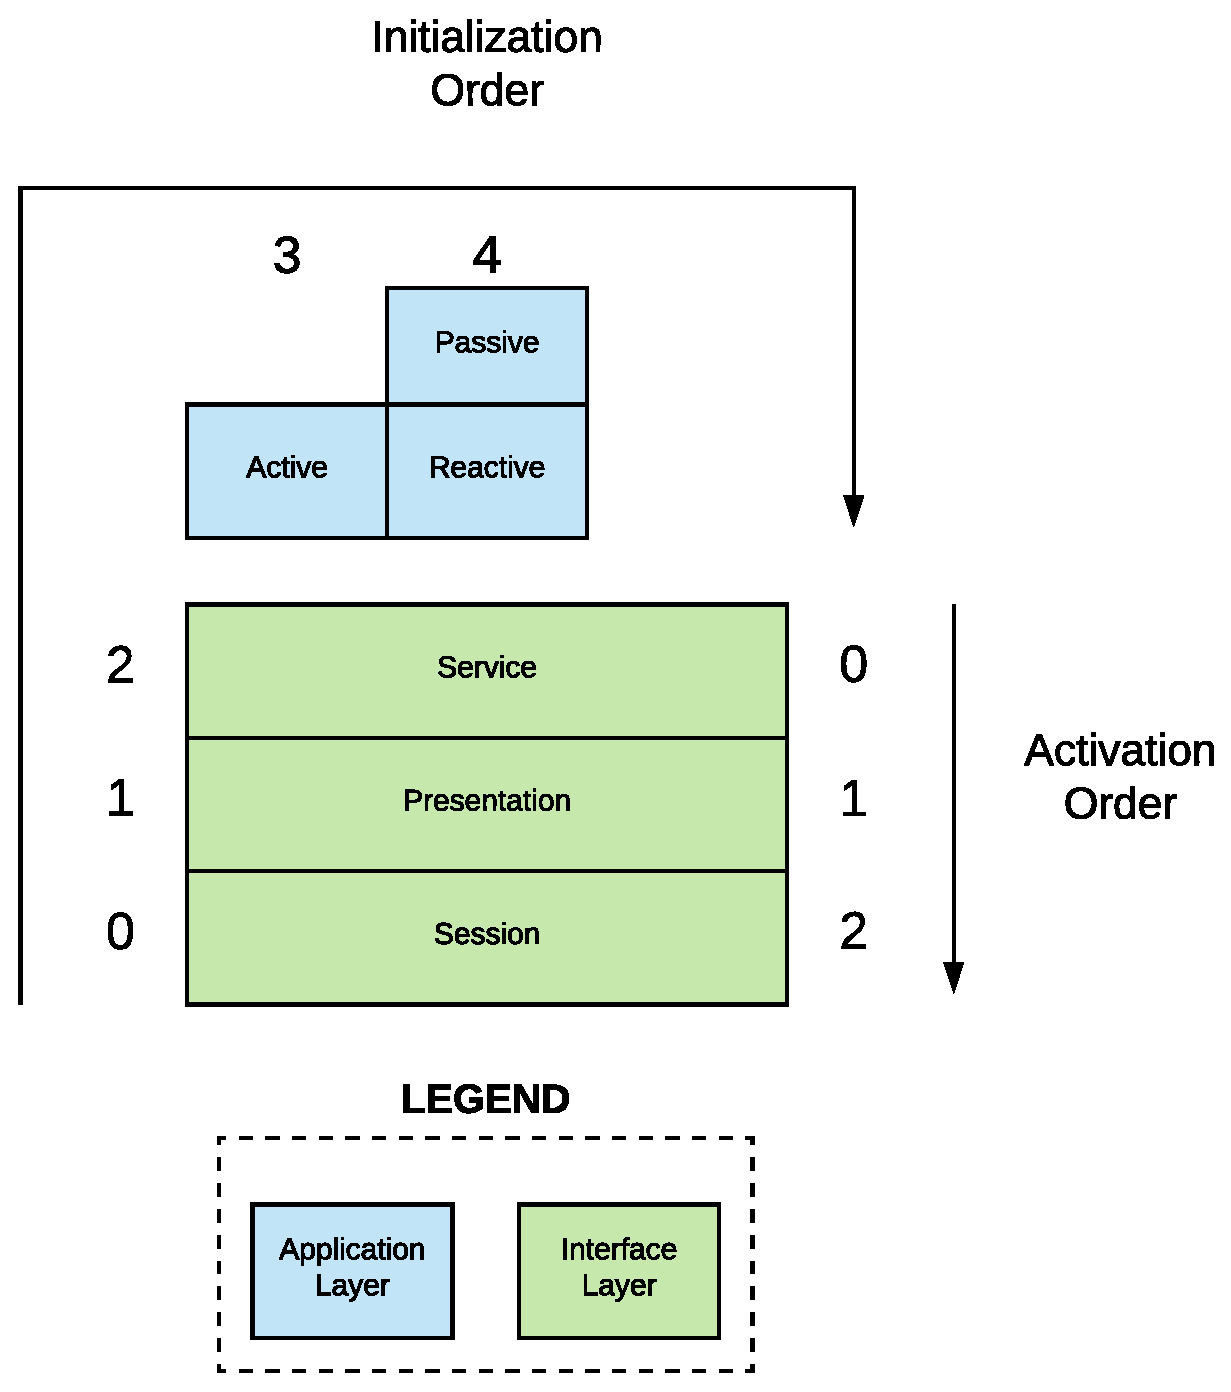
\includegraphics[scale=0.5,keepaspectratio]
    {images/solution/init_activate.eps}
  \caption{Application Bootstrap - Init}
  \label{fig:sd-app-init}
\end{figure}


\subsubsubsection{Init}

Each application node contains the \textit{Init} process,
which is the parent of all the application processes.
The execution steps of \textit{Init} are depicted in Figure
\ref{fig:sd-app-init}.
It instantiates the resources of each layer, thus making
Interface Layer and Application Layer transit from the \verb|inactive|
to the \verb|ready| state.
For example, each sublayer of Interface Layer instantiates its own pool of
LWPs\footnote{lightweight processes}.

The Application Layer initialization completes in the following order:

\begin{enumerate}
  \item \textbf{Active:} the entities which move in the city (e.g.,
    pedestrians);
  \item \textbf{Reactive:} the infrastructure of the city (e.g., streets);
\end{enumerate}

The Scheduling package, which manages the execution order for the events of the
Application Layer, does not require an initialization step. This package
will be started directly through the start message.


Since the \textit{Passive} entities are stateless and
logically belong to \textit{reactive} entities (e.g., speed limits belong to
roads), they will be instantiated along with them
(Figure \ref{fig:sd-entity-types-deps}).

When \textit{Reactive} completes its initialization, \textit{Init}
signals the Application layer completion to each sublayer of Interface Layer
in the following order:

\begin{enumerate}
  \item \textbf{Service:} provides activators and pipelines services to
    application layer;
  \item \textbf{Presentation:} provides data conversion services;
  \item \textbf{Session:} provides network connection services (e.g., senders
  and receivers).
\end{enumerate}

\textit{Init} triggers the transition of each IL sublayer state from
\verb|ready| to \verb|active|.
The activation order is extremely important to proactively avoid
message losses between remote nodes.
Indeed, at this stage, the application layer is
not able to generate or receive messages because the start message has not
been sent by the middleware. Obviously, IL is a reactive component
of the backend subystem. Thus, its \verb|active| state means
that all the workers of IL have started their event loop.
Their loop execution is triggered each time a
message arrives. Indeed, the workers are blocked on unbounded synchronized
queues which have been designed to be thread safe \cite{taft2006ada}.


The service and the presentation layer are activated before the session layer;
the latter exposes a remote communication channel through TCP
sockets.
Finally, the application is ready to communicate because both of its layers
has been activated.

Now, the Application waits the \verb|start|
message from the middleware.


A crash of the \textit{Init} process, occurring before the end of the
bootstrap, is detected by the middleware layer. The expiration
of a timeout triggers a retransmission from the middleware side.
Note that this model should also work for a bootstrap which is executed
starting
from a valid snapshot of the system, with the only difference consisting in
divergent values of the configuration file.
Indeed, for each simulation we will use a set
of configurations which is going to be different for each city.

\subsubsubsection{Start}

When \textit{Init} completes, the Application Layer is in a \verb|ready| state
while Interface Layer is in an \verb|active| state.
The first message sent by the middleware towards the Interface Layer is a
\verb|start| message which triggers the Application Layer activation.

The \verb|start| message kickoffs the scheduler, causing it to load the set
of actions declared in its configuration file. An action is a $<$\verb|agent|,
\verb|time_span|$>$ pair, i.e., the active entity \verb|agent| will act in
\verb|time_span| milliseconds.

\subsubsubsection{Termination}
When describing the shutdown of the whole system, we assumed 
the application terminates gracefully.
In this section we show the algorithm that is used to achieve this goal.

As we can see from figure \ref{fig:app-proc-tree}, the termination follows the
opposite order of the bootstrap.

\begin{enumerate}
  \item The \textit{Master} task $M$ stops active entities, e.g. pedestrians;
  \item After stopping active entities, $M$ saves their state into a file;
  \item $M$ saves into a file the state of reactive entities. 
  It is important to notice their internal state is now safetely savable, 
  since no active entities can modify it anymore;
  \item $M$ sends an \texttt{app\_shut} message to the middleware;
  \item $M$ terminates itself and the entire application consequently stops.
\end{enumerate}

The middleware layer can request the application to stop via the
\texttt{app.shutdown} call.

The last operation the \textit{Master} task does is to send a message for apprising
the middleware layer of the successful termination of the application one.
Similarly to the bootstrap phase, the middleware expects to receive this
message within a certain amount of time. 
In order to do so, when sending the message, $M$ also starts a timeout.
Wherefore if it expires before receiving a response message from the middleware layer, 
it calls again the \texttt{app.shutdown} procedure the application exposes.

\subsubsubsection{Interaction between entities}

The application contains several interactions among entities that have to be
specified in order to understand well how to approach different problems.

\paragraph{Entering a road} Moving entities enter a road by entering a stretch
that is located at the beginning of the road and that is treadable by their
specific entity type.

\paragraph{Entering a road stretch} Moving entities who want to enter a new
road stretch can do it whenever there is room for them in that stretch. In
particular, a roadway stretch can be trod for at most one vehicle at the same
time.

\paragraph{Zebra crossings} Vehicles which want to enter a road stretch that
has zebra crossings painted on it has to wait for pedestrians or bikes to free
all stretches of that particular crossing.

\paragraph{Changing roadway lane} A vehicle that is on the i-th road stretch
which wants to change lane has to check whether the (i+1)-th stretch in the
wanted direction is free.

In that case, the vehicle enters the stretch of the other lane; otherwise, if a
timeout expires before a vehicle is able to change lane, then it gives up on
it and proceeds forward to the next stretch.

\paragraph{Crossroads} Every road that is connected to a crossroads is marked
with a cardinal point (N/E/W/S). The crossroads holds all the logic necessary
for vehicles to follow the yield rules we described in
\ref{sec:pa-domain-problems}.

There could be a situation in which there is a standstill, for example when
four cars want all to go straight in a four-way crossroads. In this case, the
crossroads will make a car yield the right-of-way to another one.

Pedestrians can only walk on the corner of the crossroads, thus passing to the
adjacent piece of road (e.g. a pedestrian that is coming from the ``southern''
side of the western road can only enter the southern street on the ``western''
side).

\paragraph{Entering a building} When a moving entity is in the stretch where
there is the entrance of a building, then it may enter the building.

If the moving entity is a vehicle, it has to wait for all other entities who
are in the intermediate stretches to move away.

\paragraph{Exiting a building} When a moving entity is exiting a building, it
has to check whether there is room for her to move out.

If the entity is a vehicle, it has to yield the right-of-way to upcoming
vehicles and to wait that eventual sidewalks or bicycle path stretches in front
of the building are free too.

\paragraph{Choosing to use a vehicle} An entity $e$ who wants to leave a
building $b_e$ to a destination $d_e$ may randomly decide not to travel by
foot. She can leave only if:

\begin{itemize}
  \item the path from $b_e$ to $d_e$ does not include any destination of other
    people who are leaving from $b$ and viceversa. Otherwise, they would share
    the vehicle if there is enough room;
  \item there is an available vehicle in $b$; and
  \item the capacity of the destination building $d_e$ is greater than the sum
    of all vehicles in it and the ones which are arriving to that building.
\end{itemize}

If all these conditions are met, then:
\begin{itemize}
  \item the entity may exit the building and travel using a vehicle; and
  \item $d_e$ now ``books'' a place for the vehicle driven by $e$.
\end{itemize}

\paragraph{Waiting for a bus} A pedestrian may randomly decide to wait for a
bus if she is on a bus stop stretch.

Firstly, she checks whether the buses that stops at that stretch match (even
partially) her path. If at least one of them does, then she wait for a limited
amount of time for a bus to arrive.

If this timeout expires, then she continues travelling by foot to the next
stretch.

\paragraph{Boarding a bus} When a bus arrives at a bus stop, then a waiting
entity will board it only if:

\begin{itemize}
  \item there is enough room for her; and
  \item this bus shortens the expected route for her.
\end{itemize}

\paragraph{Getting off a bus} A person $p$ will get off a bus when it reaches
the last stop $s$ such that $s$ belongs to the route of $p$.

\paragraph{Respecting street code} Roads and crossroads will contain all the
necessary logic to make moving entities follow the street rules.

\paragraph{Performing an overtaking} This action is possible only when a
vehicle is able to change lane. It might be triggered by a timeout which
expires when it is waiting too much for entering the next straightaway stretch.

When a vehicle tries to overtake another one, it will always try to return to
the lane where it started the operation before entering the last stretch.
% look for "manovra" translation

% \paragraph{Uber} % Is it a TODO?


% Detail design
% \subsubsection{Detailed Design}

\input{sections/solutionDesign/concurrency_applicationLayer/entityType.tex}
\input{sections/solutionDesign/concurrency_applicationLayer/detail.tex}


\subsubsection{Middleware}
\subsubsubsection{Application - Middleware}
The communication protocol between application layer and middleware layer 
\paragraph{Fire and forget} 
It is a one-way message pattern (the service sends a message without expecting 
a response). Since the application and the middleware will reside on the same 
physical node we can assume that the communication is reliable, once a message 
is sent from the application layer it arrives to the middleware layer and 
viceversa. The asynchronous communication decouples (when possible) 
the computation of the application from the computation of the middleware 
and viceversa. The standard interfaces for communication 
implemented by application layer and middleware layer enables the use of 
heterogeneous technologies for each one. Defining a standard interface 
is fundamental to abstract from the underlying technologies (implementation).

\subsubsubsection{Middleware - Middleware}

The communication between the middleware layers implies the design of different 
services. Taking into account the distributed nature of the system we have 
studied specific solutions for each service, the ideas applied come from 
well known patterns used in distributed systems:
\begin{itemize}
  \item Lamport logical clocks: in a distributed system we are interested 
in the logical sequence of the events and not the wall clock time which is 
impossible to know perfectly and could lead to synchronization errors;
  \item Lamport timestamps algorithm\footnote{Leslie Lamport \textit{Time, 
clocks, and the ordering of events in a distributed system}, ACM 21, 
pp. 558-565, July 1978}: this algorithm contains the keystone 
of each distributed service which implies a form of synchronization 
between parties;
  \item Bully algorithm: this algorithm is used in the first part of the 
shutdown process. It works dynamically and implies the election of a master 
node. 
\end{itemize}

\subsubsubsection{System Boostrap}
As pointed out in Problem Analysis (\ref{sec:pa-distribution}), the system has
to start neatly. Hence, we need to design a protocol in order to accomplish 
this goal.

The protocol is represented in figure \ref{fig:sys-bootstrap-protocol}, where:

\begin{itemize}
  \item A circle is a logical node which is composed of two layers:
    \begin{itemize}
      \item \textbf{MW}:  middleware layer
      \item \textbf{APP}: application layer
  \end{itemize}
    Since the middleware has to be application-independent, it only assumes 
    that the application layer exposes an interface through which it is 
    possible to start the application neatly;
  \item \textbf{Named arrow}: it represents a message that is sent from a 
logical node through another one with the name as its payload;
  \item \textbf{Number}: it represents the progress of the logical system clock 
during the bootstrap process.
\end{itemize}

\begin{figure}[H]
  \centering
  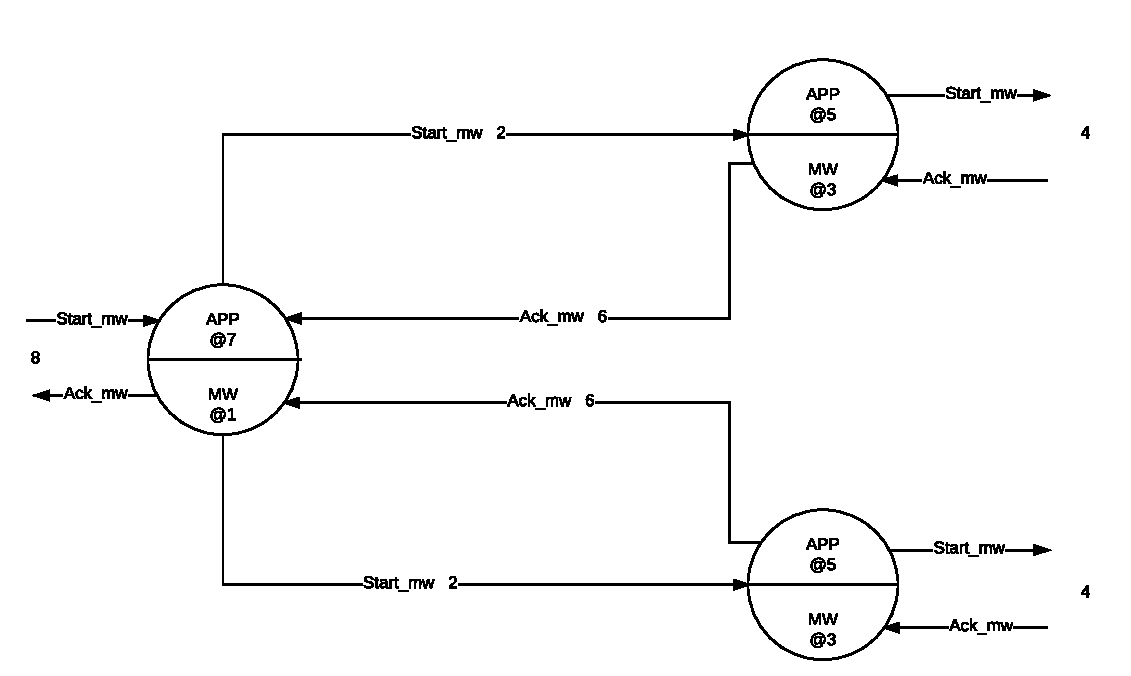
\includegraphics[width=\columnwidth]{sections/images/solution/bootstrap.pdf}
  \caption{System bootstrap protocol}
  \label{fig:sys-bootstrap-protocol}
\end{figure}

Assuming that a \texttt{Start\_mw} message arrives to a non-booted node (say
$l$) at time 0, the protocol is defined as follows:

\begin{enumerate}
  \item The leftmost node $l$ in figure \ref{fig:sys-bootstrap-protocol}
    starts its own middleware services.  
  \item $l$ sends a \texttt{Start\_mw} message to the set $S$ of all its
    neighbors. Clearly, if it was the first node in the system to receive
    \texttt{Start\_mw}, then it will be also the last node to complete the
    boot process.
  \item $l$ waits for each node in $S$ to complete the boot. $l$ waits for all
nodes in $S$ to send an \texttt{Ack\_mw} message back;
  \item The middleware MW of $l$ grants the application APP to start;
  \item $l$ then sends an \texttt{Ack\_mw} message back.
\end{enumerate}

As it can be seen in the figure, this behaviour is replicated recursively
by all nodes of the system. If a node has already been booted, then it only
sends \texttt{Ack\_mw} back.

\subsubsubsection{System Termination}
Also, the system has to shutdown neatly. Therefore we designed a protocol to
stop the entire system; please notice that this one could be seen as a
symmetric version of the System Bootstrap protocol.
% TODO: please check the sentence here above

The protocol is represented in figure \ref{fig:sys-termination-protocol}, where
the conventions are the same as the ones used in figure
\ref{fig:sys-bootstrap-protocol}.

\begin{figure}[H]
  \centering
  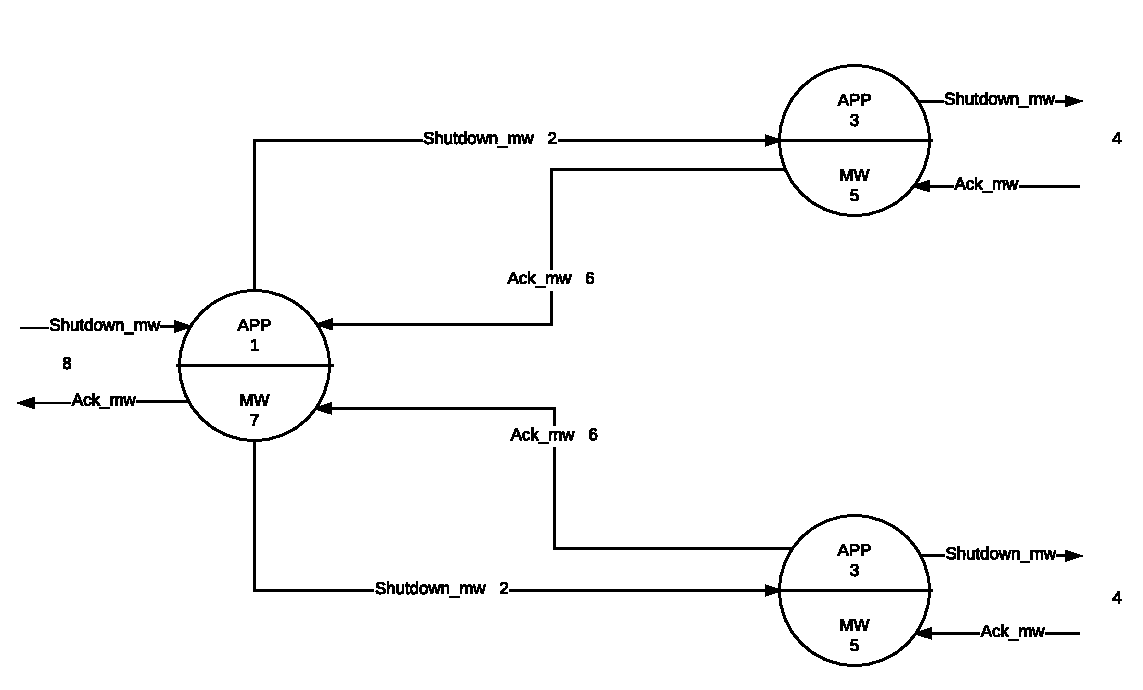
\includegraphics[width=\columnwidth]{sections/images/solution/termination.pdf}
  \caption{System termination protocol}
  \label{fig:sys-termination-protocol}
\end{figure}

Assuming that a \texttt{Shutdown\_mw} message arrives to a non-terminated node
$l$ (let it be the leftmost one in the picture) at time instant 0, the protocol
is defined as follows:

\begin{enumerate}
  \item The middleware MW of $l$ asks to terminate the application APP;
  \item $l$ sends a \texttt{Shutdown\_mw} message to the set
    $S$ of all the nodes it knows;
  \item $l$ waits for each node in $S$ to terminate, i.e. $l$ waits for all
    nodes in $S$ to send an \texttt{Ack\_mw} message back;
  \item $l$ stops its own middleware services;
  \item $l$ then sends an \texttt{Ack\_mw} message back.
\end{enumerate}

As it can be seen in the related figure, this behaviour is replicated
recursively by all nodes of the system. If a node has already terminated, then
it only sends \texttt{Ack\_mw} back.



% Artificial Intelligence subsection
\subsection{Broker}

We decided to put an intermediate broker between the middleware(s) and the
application server(s) to make our system more scalable.

Indeed, the messages sent by the middleware have two deficiencies:

\begin{enumerate}
  \item \textit{Size} -- middleware messages carry a significant amount of
    information, because middleware does not perform deep inspection of the
    payload (the application domain is completely transparent) and, therefore,
    messages are forwarded as they are received from the upper application
    layer;
  \item \textit{Poor semantics} -- middleware outputs events with its best
    effort, but it can only read the headers of application layer messages.
    Therefore, message topics are just a concatenation of little detailed
    information obtained by the application.
\end{enumerate}

Our message broker tries to overcome these problems by performing deep
inspection on the payloads of the messages, filtering information from them and
building more meaningful topics for the messages (we will provide more details
in Section \ref{sec:impl-broker}).


% Artificial Intelligence subsection
\subsection{Artificial Intelligence (AI)}

Our AI offers three path finding algorithms:
\begin{itemize}
  \item Greedy Search;
  \item Uniform Cost Search;
  \item A* Search.
\end{itemize}

The first one is incomplete and not optimal because of the local search which looks only one step ahead (visiting
only the neighbors). The last two algorithm are both complete and optimal under certain assumptions. They have been defined
to guarantee our agents to always find the best possible path with the minimum number of visited nodes in the search graph.

To guarantee completeness we need to assume that each graph is a strongly
connected component. Basically, it means that there are no isolated
components. Thus, the agent knows there will always be at least a path between
the source and the destination of its plan. % its or her

Furthermore, our AI considers not grid based maps: which means some common
heuristics are not applicabile a priori (e.g. Manhattan distance, euclidean
distance). Also, since grid-based maps are a subset of all possible maps, we
can say that our AI is independent on the map toopology.

To solve the path finding problem we reason about the specific domain and its
abstractions in terms of infrastructure building blocks and travellers. We
found an admissibile and consistent heuristic for A* and in general other
informed algorithms. To concretely guarantee the assumptions hold for all the
graph configurations we apply the Tarjan algorithm.

Tarjan automatically validates our graphs at build time by ensuring that there
is only one strong connected component for each graph, otherwise it reports
an error and shows the isolated component.
Finally, the AI is agent-independent, which means we can use it to calculate
the path of different kinds of agents: bicycles which move on bicycle lanes,
pedestrians who move on sidewalks and motor vehicles which move on roads.


